\section{ XML路径语言XPath}

\begin{frame}[fragile]{CH6 XML路径语言XPath}
\begin{figure}
    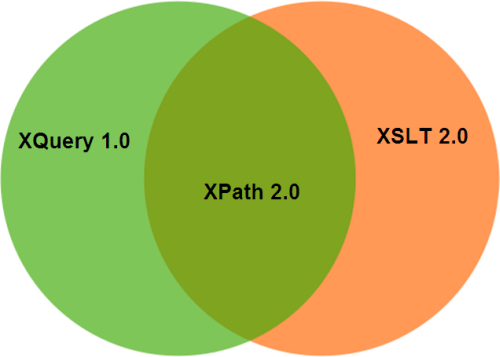
\includegraphics[width=0.5\textwidth]{figure/xpath.png}
\end{figure}
\end{frame}

\begin{frame}[fragile, allowframebreaks]{本章学习目标}
\begin{easylist} \easyitem
& 了解XPath的工作原理
& 掌握XPath的定位路径表达式
& 熟悉XPath的常用函数和数据类型
& 掌握XPath2.0的部分新特性
\end{easylist}
\end{frame}

\begin{frame}[fragile, allowframebreaks]{目录}
\begin{easylist} \easyitem
& XPath概述
&& XPath及其作用
&& XPath工作原理
&& XPath的表达式与操作符
&& 如何测试XPath

& XPath结点与结点集
&& 结点的基本属性
&& 结点类型
&& 结点集

& XPath定位路径表达式
&& XPath定位步骤
&& XPath轴
&& 结点测试
&& 谓词
&& 定位路径缩写

& XPath的基本表达式
&& 布尔表达式
&& 等式表达式
&& 关系表达式
&& 数值表达式

& XPath数据类型
&& 字符串类型
&& 数值类型
&& 布尔类型
&& 结点集类型

& XPath 1.0常用函数
& XPath 2.0
\end{easylist}
\end{frame}


\subsection{6.1 概述}

\begin{frame}[fragile]{6.1 概述}
\begin{easylist} \easyitem
& 考虑以下问题
&& 从存储图书信息的XML文档中选择指定ISBN号码的图书标题信息
&& 从XML文档中排除掉某些信息再进行处理
&&& 例如:当显示员工信息时,把工资信息隐藏掉不予显示
&& \em{如何从XML文档中选择部分结点或结点集合,实现对XML文档中的元素、属性等信息的定位和查找,准确快速的找到XML文档结构树中的任意一个或一组结点}
\end{easylist}
\end{frame}


\subsubsection{6.1.1 XPath及其作用}
\begin{frame}[fragile]{6.1.1 XPath及其作用}
\begin{easylist} \easyitem
& XPath
&& XML Path Language
&& 把整个XML文档看成是一棵由结点组成的层次树,通过结点路径进行定位
&& XPath 1.0
&&& 1999年11月16发布,作为XSLT和XPointer的配套标准,用于XML文档的寻址
&& XPath 2.0
&&& XPath 1.0的超集,增加了丰富的数据类型
\end{easylist}
\end{frame}


\begin{frame}[fragile]{6.1.1 XPath及其作用}
\begin{easylist} \easyitem
& XPath的作用
&& XPath为XML文档提供一种快捷方便并易于使用的寻址功能,实现对XML文档树中指定结点或结点集合的选择定位。
&& XPath为XML其他相关技术提供核心支持,包括XSLT、XQuery、XPointer、XForm等。
&& XPath为人们处理XML文档提供了一种标准通用规范,XPath的公共API接口独立于特定语言,使得对XML文档的操纵处理更为方便
\end{easylist}
\end{frame}


\subsubsection{6.1.2 XPath的工作原理}
\begin{frame}[fragile]{6.1.2 XPath的工作原理}
\begin{easylist} \easyitem
& 从内容构成来看,XML文档与普通的文本文件相同,因此又称为序列化XML文档(Serialized XML Document)
& XML更注重逻辑结构特征,目前三个从不同角度描述XML文档的逻辑模型
&& XPath
&& DOM
&& XML信息集合(XML Information Set)
\end{easylist}
\end{frame}


\begin{frame}[fragile]{XPath数据模型}
\begin{easylist} \easyitem
& XPath把XML文档看成是一个或一组文档树结点,文档的大部分内容都表示为结点
& XML文档的特殊部分没有对应的XPath表示方式
&& 例如:最开始的XML声明语句
\end{easylist}
\end{frame}


\begin{frame}[fragile]{文档对象模型DOM}
\begin{easylist} \easyitem
& 同样把整个XML文档表示成一棵由结点组成的层次树
& DOM和XPath在表示结点的方式上有所不同
&& DOM中的结点包含有丰富的信息,更多的应用于XML编程处理方面
&& 例如DOM结点对象有类型、属性、方法等概念
\end{easylist}
\end{frame}


\begin{frame}[fragile]{XML信息集合}
\begin{easylist} \easyitem
& 也叫XML信息集
& XML信息集是XML文档的纯信息表示,适用于从XML角度而非文本角度比较两个文件的异同
&& 信息集不区分空元素的两种形式
&& 属性所使用的引号类型也不重要,克服了严格的文本字符比较的缺点
\end{easylist}
\end{frame}


\begin{frame}[fragile, allowframebreaks]{文本不同但信息集合角度相同的两个XML文档}
\begin{lstlisting}[tabsize=8, basicstyle=\small\tt, language=XML, caption=''6-1.xml'']
<?xml version="1.0" encoding="UTF-8"?>
<order id="TEST-01">
    <?backup dbname="order"?>
    <product name="打印纸" price="30" quantity="5"/>
    <product name="圆珠笔" price="2" quantity="10"/>
    <product name="铅笔" price="1.5" quantity="10"/>
    <product name="白板" price="80" quantity="2"/>
</order>
\end{lstlisting}

\newpage
\begin{lstlisting}[tabsize=8, basicstyle=\small\tt, language=XML, caption=''6-2.xml'']
<order id='TEST-01' >
    <?backup dbname="order"?>
    <product name='打印纸' price='30' quantity='5'/>
    <product name='圆珠笔' price='2' quantity='10'/>
    <product name='铅笔' price='1.5' quantity='10'/>
    <product name='白板' price='80' quantity='2'/>
</order>
\end{lstlisting}
\end{frame}


\begin{frame}[fragile]{XPath}
\begin{figure}
    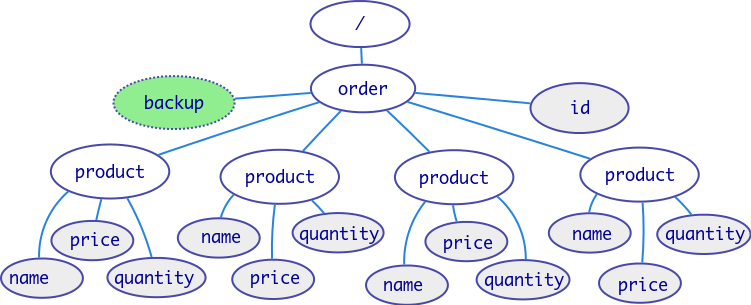
\includegraphics[width=0.75\textwidth]{figure/xpath-tree.png}
\end{figure}
\begin{easylist} \easyitem
& 利用结点之间的层次关系实现定位
& 例子:
\begin{lstlisting}[tabsize=8, basicstyle=\small\tt, language=XML, numbers=none]
/order/product[2]/@name
\end{lstlisting}
\end{easylist}
\end{frame}


\subsubsection{6.1.3 XPath的表达式与操作符}
\begin{frame}[fragile]{6.1.3 XPath的表达式与操作符}
\begin{table}[!hbp] 
\begin{tabular}{l|l}
\Xhline{1.3pt}
表达式类型 &	操作符 \\ \Xhline{1.3pt}
定位路径表达式& /,  //,  |  \\ \hline
布尔表达式 & or,   and  \\ \hline
等式表达式 & =,   !=  \\ \hline
关系表达式 &	<=,  <,  >=,  >  \\ \hline
数值表达式 & 	+,  -,  div,  mod,  *,  -(unary)  \\ \hline
\end{tabular}
\end{table}
\end{frame}


\subsubsection{6.1.4 如何测试XPath}
\begin{frame}[fragile]{6.1.4 如何测试XPath}
\begin{figure}
    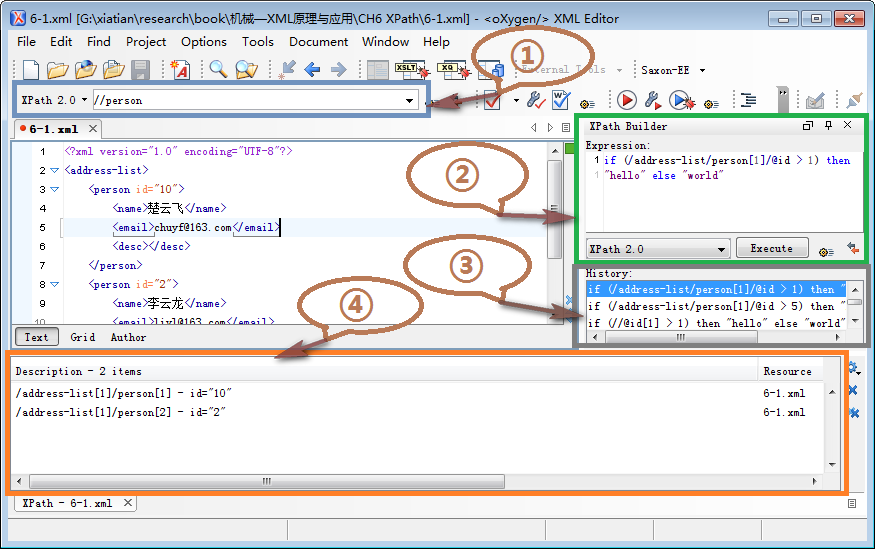
\includegraphics[width=0.85\textwidth]{figure/xpath-test-oxygen.png}
\end{figure}
\end{frame}



\subsection{6.2 XPath结点与结点集}
\begin{frame}[fragile]{6.2 XPath结点与结点集}
\begin{easylist} \easyitem
& 结点可看成是XPath定位步中用来实现定位功能的离散的、逻辑性的东西
&& XML文档中的任意一个元素、属性、处理指令、注释等,都可以是一个结点
& 结点集:结点组成的集合
\end{easylist}
\end{frame}


\subsubsection{6.2.1 结点的基本属性}
\begin{frame}[fragile]{6.2.1 结点的基本属性}
\begin{easylist} \easyitem
& 结点名称
& 结点顺序
& 结点之间的家族关系
\end{easylist}
\end{frame}


\begin{frame}[fragile]{结点名称}
\begin{easylist} \easyitem
& 大部分结点都用名称(根结点没有),三种名称:
&& 限定名称QName(Qualified name)
&&& XML文档实例中该结点的唯一标识符,包括结点的命名空间前缀部分
&&& <product>元素的QName为product
&&& <common:product>的QName为common:product

&& 本地名称(Local-name)
&&& QName去除命名空间前缀后剩余的内容
&&& 如果没有指定命名空间,其规范名称和本地名称完全相同
&&& <common:product>的本地名称为product

&& 扩展名称(Expended-name)
&&& 扩展名称由与命名空间关联的URI与本地名称共同构成
&&& 扩展名称不关心命名空间前缀的具体名称
\end{easylist}
\end{frame}


\begin{frame}[fragile]{结点顺序}
\begin{easylist} \easyitem
& 结点位置是由该结点前面的结点和后面的结点所决定的
& 通常按照先后顺序进行访问
& 借助于XPath坐标轴,也可以实现对XML文档结点的逆序访问或指定顺序访问
\end{easylist}
\end{frame}


\begin{frame}[fragile]{结点之间的家族关系}
\begin{easylist} \easyitem
& 结点之间通过XPath坐标轴维持关系
& 常见关系包括:
&& 相邻关系
&& 祖先关系
&& 子孙关系
&& ...
\end{easylist}
\end{frame}


\subsubsection{6.2.2 结点类型}
\begin{frame}[fragile]{6.2.1 结点的基本属性}
\begin{easylist} \easyitem
& 根节点
& 元素节点
& 属性节点
& 命名空间节点
& 处理指令节点
& 注释节点
& 正文节点
\end{easylist}
\end{frame}


\subsubsection{6.2.3 结点集}
\begin{frame}[fragile]{6.2.3 结点集}
\begin{easylist} \easyitem
& 由结点构成的集合
& 例如“6-1.xml”中,位置路径/order/product则返回一个包含了4个product元素的结点集
\end{easylist}
\end{frame}



\subsection{6.3 XPath定位路径表达式}
\begin{frame}[fragile]{6.3 XPath定位路径表达式}
\begin{easylist} \easyitem
& 由一个或多个定位步骤组成,每个定位步骤之间用斜线“/”分隔
& 如表达式以“/”开始,则称为绝对路径,否则称为相对路径
& 使用“/”符号作为定位步骤之间的分隔符
\end{easylist}
\end{frame}


\subsubsection{6.3.1 XPath定位步骤}
\begin{frame}[fragile]{6.3.1 XPath定位步骤}
\begin{easylist} \easyitem
& 定位步骤的组成
&& 轴:用来导航XPath数据模型的结点树的工具
&& 测试结点:用来确定选取轴中哪类结点
&& 谓词:可选步骤,用来过滤轴和定位方法所选取的结点集
\end{easylist}
\begin{figure}
    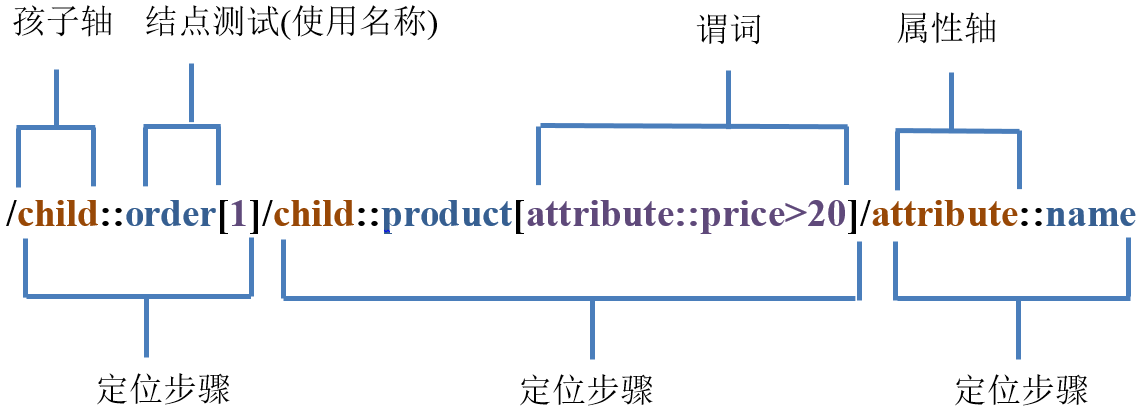
\includegraphics[width=0.75\textwidth]{figure/xpath-step.png}
\end{figure}
\end{frame}


\subsubsection{6.3.2 XPath轴}
\begin{frame}[fragile]{6.3.2 XPath轴: 在结点的哪一个方向上进行导航定位}
\begin{table}[!hbp] 
\begin{tabular}{l|l|l}
\Xhline{1.3pt}
轴 & 名称 & 方向  \\ \Xhline{1.3pt}
child & 子轴 & 前向 \\ \hline
parent & 双亲轴 & 不可用 \\ \hline
attribute & 属性轴 & 不可用 \\ \hline
ancestor & 祖先轴 & 反向 \\ \hline
ancestor-or-self & 祖先自身轴 & 反向 \\ \hline
descendant & 子孙轴 & 前向 \\ \hline
descendant-or-self & 子孙自身轴 & 前向 \\ \hline
following & 后继轴 & 前向 \\ \hline
following-sibling & 后继兄弟轴 & 前向 \\ \hline
preceding & 前驱轴 & 反向 \\ \hline
preceding-sibling & 前驱兄弟轴 & 	反向 \\ \hline
namespace & 命名空间轴 & 不可用 \\ \hline
self & 自身轴 & 不可用 \\ \hline
\end{tabular}
\end{table}
\end{frame}



\begin{frame}[fragile, allowframebreaks]{XPath轴示例}
\begin{easylist} \easyitem
& 示例文档
\begin{lstlisting}[tabsize=8, basicstyle=\small\tt, language=XML]
<?xml version="1.0" encoding="UTF-8"?> 
<abc:order id="TEST-01" xmlns:abc="http://www.abc.com" 
                    xmlns:abc2="http://www.abc2.com">
    <?backup dbname="order"?>
    <product name="打印纸" price="30" quantity="5"/>
    <product name="圆珠笔" price="2" quantity="10"/>
    <product name="铅笔" price="1.5" quantity="10"/>
    <product name="白板" price="80" quantity="2"/>
</abc:order>
\end{lstlisting}

\newpage
& 测试表达式:
\begin{lstlisting}[tabsize=8, basicstyle=\small\tt, language=XML, numbers=none]
/abc:order/namespace::abc
\end{lstlisting}

& 结果:
\begin{lstlisting}[tabsize=8, basicstyle=\small\tt, language=XML, numbers=none]
abc - http://www.abc.com
\end{lstlisting}

& 测试表达式:
\begin{lstlisting}[tabsize=8, basicstyle=\small\tt, language=XML, numbers=none]
/abc:order/namespace::node()
\end{lstlisting}

& 结果:
\begin{lstlisting}[tabsize=8, basicstyle=\small\tt, language=XML, numbers=none]
xml - http://www.w3.org/XML/1998/namespace
abc - http://www.abc.com
abc2 - http://www.abc2.com
\end{lstlisting}
\end{easylist}
\end{frame}


\subsubsection{6.3.3 结点测试}
\begin{frame}[fragile]{6.3.3 结点测试}
\begin{easylist} \easyitem
& 用于确定轴中的结点,只有给定结点的结点测试结果为true,该结点才会保留在结点集中
& 使用名称进行测试,例如:
&& child::brandA:product
&& 选中QName为brandA:product的所有孩子元素结点
& 使用类型进行测试,例如:
&& child::text( )	
&& 确定文本子结点
& 参考教材内容
\end{easylist}
\end{frame}


\subsubsection{6.3.4 谓词}
\begin{frame}[fragile]{6.3.4 谓词}
\begin{easylist} \easyitem
& 谓词是指针对条件表达式进行求值返回真或假的过程
& 谓词置于定位步骤末端的方括号中,用于筛选一个结点集以生成新的结点集
& 针对结点集中每一个被筛选的结点,谓词表达式将此结点作为上下文结点进行求值,如为true,则保留在结点集中,否则,从结点集中删除
& 例子:
&& descendant::product[attribute::price > 20]	
&& 选择product的子孙元素,且product元素拥有大于20的price属性
\end{easylist}
\end{frame}


\subsubsection{6.3.5 定位路径缩写}
\begin{frame}[fragile]{6.3.5 定位路径缩写}
\begin{table}[!hbp] 
\begin{tabular}{l|l}
\Xhline{1.3pt}
示例 & 对应缩写示例 \\ \Xhline{1.3pt}
child::product & product \\ \hline
child::product/attribute::name & product/@name \\ \hline
self::node()/product & ./product \\ \hline
parent::node()/@name & ../@name \\ \hline
/descendant-or-self::node()/product & //product \\ \hline
child::product[position( ) == 3] & product[3] \\ \hline
\end{tabular}
\end{table}
\end{frame}



\subsection{6.4 XPath基本表达式}
\begin{frame}[fragile]{6.4 XPath基本表达式}
\begin{easylist} \easyitem
& 布尔表达式:and or
&& person[name and age]
&& person[(age>30) or (age<50)]
& 等式表达式: =, !=
&& age = 30
&& age != 30
& 关系表达式:<, <=, >, >=
&& age <= 30
& 数值表达式:+, -, div, mod, * -(unary)
&& person[(age mod 2) =0]
&& 选择具有偶数数值age子元素的person子元素
\end{easylist}
\end{frame}



\subsection{6.5 XPath数据类型}
\begin{frame}[fragile]{6.5 XPath数据类型}
\begin{easylist} \easyitem
& 字符串类型
&& person[name='李云龙']
& 数值类型
&& <pages>102</pages>
&& pages + 10
& 布尔类型
&& order[@id="1"]
& 结点集类型、
&& //book
\end{easylist}
\end{frame}


\subsection{6.6 XPath 1.0常用函数}
\begin{frame}[fragile]{6.6 XPath 1.0常用函数}
\begin{easylist} \easyitem
& 结点集相关函数
& 布尔函数
& 数值函数
& 字符串函数
\end{easylist}
\end{frame}


\subsection{6.6.1 结点集函数}
\begin{frame}[fragile]{6.6.1 结点集函数}
\begin{easylist} \easyitem
& last()
&& 返回上下文的大小,即给定上下文中的节点数。
& position()
&& 返回上下文结点的位置。比如,可以用表达式 position()=last() 测试处理的是否是集合中最后一个节点。
& count()
&& 参数为结点集,返回这个结点集中包含的结点个数。
& id()
&& 参数为字符串,返回一个结点集,结点集中的每一个结点的ID属性值等于这个参数字符串。
XPath中的另外三个与结点集相关的函数为:
\end{easylist}
\end{frame}


\subsection{6.6.2 布尔函数}
\begin{frame}[fragile]{6.6.2 布尔函数}
\begin{easylist} \easyitem
& boolean()
&& 以对象为参数,返回一个布尔值。当参数是一个非0数值时,返回true,为数值0时,返回false;当参数为字符串时,返回true;如参数为结点集并且非空,返回true,否则为false。
& not()
\end{easylist}
\end{frame}


\subsection{6.6.3 数值函数}
\begin{frame}[fragile]{6.6.3 数值函数}
\begin{easylist} \easyitem
& number ()
&& 把可选的对象参数转化成数字
& sum ()
&& 以结点集为参数,把每个结点值转换为数值,再求和返回
& ceiling ()
&& 参数为一个数值,返回比该数值大的最小整数
& floor ()
&& 参数为一个数值,返回比该数值小的最大整数
& round ()
&& 参数为一个数值,返回和参数最接近的整数
\end{easylist}
\end{frame}


\subsection{6.6.4 字符串函数}
\begin{frame}[fragile]{6.6.4 字符串函数}
\begin{easylist} \easyitem
& string ()
&& 参数可以是任何类型,返回它们的字符串值。
& string-length ()
&& 参数为一个字符串,返回该字符串长度。
& substring ()
& concat ()
& contains ()
& starts-with ()
\end{easylist}
\end{frame}



\subsection{6.7 XPath 2.0}
\begin{frame}[fragile, allowframebreaks]{6.7 XPath 2.0}
\begin{easylist} \easyitem
& 2007年1月23日正式成为推荐标准
& 新特性
&& 支持XML Schema的数据类型
&& 提供了更为丰富的处理函数
&&& tokenize():拆分字符串,
&&& matches():测试字符串是否匹配
&&& current-date()
&& 支持序列
&&& 例子:
\begin{lstlisting}[tabsize=8, basicstyle=\small\tt, language=XML, numbers=none]
for  $i  in  1 to 6  return  $i*$i
\end{lstlisting}
&&& 该表达式会生成序列(1,4,9,16,25,36)
\newpage
&& 支持逻辑判断
\begin{lstlisting}[tabsize=8, basicstyle=\small\tt, language=XML, numbers=none]
if( sum(for $p in //product return $p/@price*$p/@quantity)  > 200) then "YES" else "NO"
\end{lstlisting}
&&& 针对例6-5中的XML文档,输出结果为”YES“
&& 提供了更多的结点测试函数
&&& //element(): 选取文档中的全部元素结点
&&& //attribute():选择所有的属性结点
&& 可以调用自定义函数
&&& XPath2.0本身并不能建立自定义函数,只能在支持XPath的XSLT、XQuery等应用程序中建立自定义函数,供XPath调用
\end{easylist}
\end{frame}

\begin{frame}
\begin{center}
    \Huge END
\end{center}
\begin{figure}
    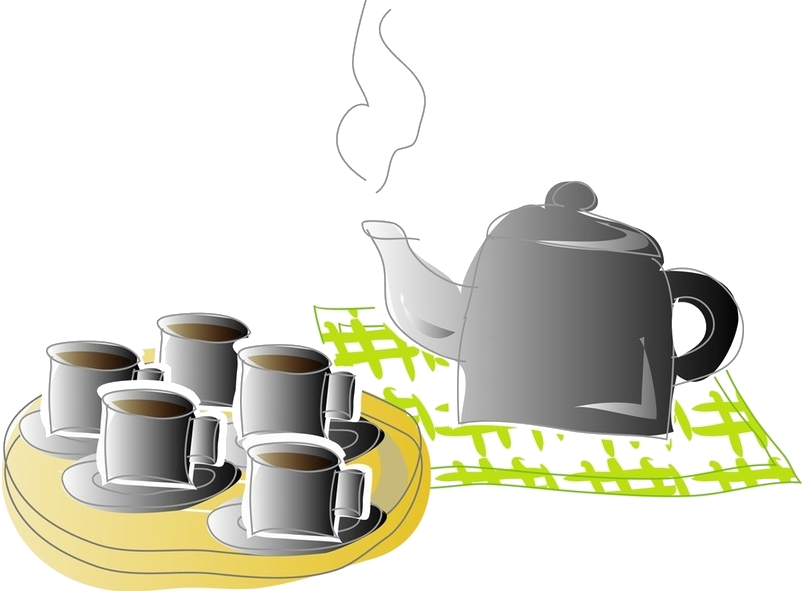
\includegraphics[width=0.75\textwidth]{figure/relax.png}
\end{figure}
\end{frame}
